\chapter{Simulations}
To see if the FHTBoost algorithm developed actually works, we need to test it on simulated data. In this chapter we describe two scenarios,
and for each, use the algorithm to estimate a model, and see how it performs. The scenarios are both thought to be realistic scenarios
where one has clinical measurements, in a high-dimensional covariate matrix $\X$, as well as gene expressions,
in a low-dimensional covariate matrix $\Z$. We link each covariate to a parameter in a parameter vector,
where $\X$ corresponds to $\bbeta$, and $\Z$ corresponds to $\bgamma$. In each parameter vector, we set a small number of parameters
to a non-zero value, and all the rest to zero. This means that only a very small number of covariates have an effect.
Given parameter vectors and covariate matrices, we can calculate a specific $y_0$ and a $\mu$ for each individual.
We draw an observation from the inverse gaussian distribution with these parameters.

We use the FHTBoost algorithm to estimate the parameter vector

We have discussed the importance of a test set, and of finding an appropriate $\mstop$. Since we are simulating, we can generate a test set
by drawing from a seed, and we therefore made the test set quite big, with $N_{\text{test}}=1000$ observations.

We generate $B\approx500$ data sets by drawing FHT data according to algorithm X. Each data set has $N=500$ observations. 
We treat each data set as a separate training data set, and thus estimate $B$ models.
To estimate each model, we first perform repeated 5-fold cross validations, with 5 repeats, on the training data set.
As shown in section ..., this should provide a reasonably stable $\mstop$ (near the ``true'' $\mstop$) for that specific data set.
We then estimate a model on the test set, by running FHTBoost with $\mstop$ number of iterations. We record metrics on these,
concerning variable selection and log-likelihood (loss function) performance.

\section{Variable selection metrics}
As mentioned in section ..., a component-wise algorithm, such as FHTBoost, performs data-driven variable selection.
We wish to see how the boosting algorithm performs, does it select informative variables and make sure not to select non-informative ones? 
In a given estimated boosting model, the model has selected a certain amount of variables.
We denote a selected variable as a ``positive,'' or $P$ for short, and a variable which is not selected as ``negative'', or $N$ for short.
Since we know which variables actually affect the response, we know how many of the variables selected are selected correctly, in the sense
that they are selected and they have an effect. We call these true positives, or $TP$ for short.
Similarly, we know which variables do not affect the response, and so we can calculate the number of non-informative variables
which were not selected, i.e., true negative, or $TN$ for short. Furthermore, we say that variables which have been selected
but which do not actually have an effect, are false positives, $FP$. Finally, false negatives, $FN$, are variables which do actually
have an effect, but which were not selected in the boosting model.

\subsection{Sensitivity}
Ideally, this is 1.
\begin{equation}\label{eq:sensitivity}
    \text{Sensitivity}=\frac{TP}{P}
\end{equation}

\subsection{Specificity}
Ideally, this is 1.
\begin{equation}\label{eq:specificity}
    \text{Specificity}=\frac{TN}{N}
\end{equation}

\subsection{Accuracy}
Ideally, this is 1.
\begin{equation}\label{eq:sensitivity}
    \text{ACC}=\frac{TP+TN}{P+N}
\end{equation}

\subsection{False positive rate}
Ideally, this is 0.
\begin{equation}\label{eq:sensitivity}
    \text{FPR}=\frac{FP}{N}.
\end{equation}

\subsection{False negative rate}
Ideally, this is 0.
\begin{equation}\label{eq:sensitivity}
    \text{FNR}=\frac{FN}{P}
\end{equation}

\section{Large simulation with uncorrelated matrices}
Here, $N$ is 500. We let $\bbeta$ be a large vector of size $p=10001$, and $\bgamma$ be a small vector of size $d=16$. Specifically, we set the intercept term in $\bbeta$ to be 2.0, and the first 35 elements to be 0.1. We set the rest to be 0. For $\bgamma$, we set the intercept term to be -1, and in similar fashion, let the first 5 elements have a non-zero value of -0.1. Here also we set the remaining 10 elements to be 0. So,
\begin{align*}
    \bbeta=\left(2.0, \underbrace{0.1, 0.1, \ldots, 0.1}_{\text{length 35}}, \overbrace{0, 0, \ldots, 0}^{\text{length 9965}}\right) \\
    \bgamma=\left(-1.0, \underbrace{0.1, 0.1, \ldots, 0.1}_{\text{length 5}}, \overbrace{0, 0, \ldots, 0}^{\text{length 10}}\right)
\end{align*}
We draw $X$ and $Z$ from 

To make a test set, we draw $N_{\text{test}}=1000$ lifetimes from a distribution with the same parameters, but of course with a unique seed.
\todo[inline]{add Kaplan-Meier plot}

With this exact setup, we run a simulation experiment $B=500$ times, where we at the beginning of each simulation set the seed, via \verb|set.seed(seed)| to be $b=1,\ldots,B$. We first generate matrices $X$ and $Z$, and simulate FHT times from the algorithm above. We then run cross validation on this data set to find the optimal iteration number $m_{\text{stop}}$. Below is a box plot of the resulting times. We then run a boosting algorithm with $m_{\text{stop}}$ steps on the training set, and use the resulting model on the test set.

\subsection{Deviance}
The difference in deviance between a fitted model and the null model containing no covariates is given by
\begin{equation*}
    d=-2\left(l^{\text{test}}(\beta_{\text{train}})-l^{\text{test}}(0)\right),
\end{equation*}
where $l^{\text{test}}(\beta)$ is the likelihood attained with covariate vector $\beta$ on the test set.

\subsection{Boosting with changing the intercept}
See Table \ref{table:non-correlated-with-intercept-summary}, Table \ref{table:non-correlated-with-intercept-y0}, and \ref{table:non-correlated-with-intercept-mu}.
\begin{table}\caption{Summary of results}\label{table:non-correlated-with-intercept-summary}
\begin{tabular}{l|rrrr}
Measure &   Mean & Standard deviation &  Minimum &    Maximum \\
\hline
Deviance    &    91.955 & 41.760 &    -7.191 &   233.563 \\
$\mstop$      &    15.823 &  6.435 &     2 &    39 \\
Log-likelihood      & -2325.746 & 20.363 & -2382.825 & -2270.023 \\
Null model log-likelihood & -2371.723 &  3.935 & -2396.848 & -2368.769
\end{tabular}
\end{table}

\begin{table}\caption{Result for $y_0$, $\beta$}\label{table:non-correlated-with-intercept-y0}
\begin{tabular}{l|rr}
Measure &  Mean &    Standard deviation \\
\hline
Sensitivity & 0.187 & 0.092 \\
Specificity & 1.000 & 0.000 \\
Accuracy    & 0.997 & 0.000 \\
False positive rate & 0.000 & 0.000 \\
False negative rate & 0.813 & 0.092
\end{tabular}
\end{table}


\begin{table}\caption{Result for $\mu$, $\gamma$}\label{table:non-correlated-with-intercept-mu}
\begin{tabular}{l|rr}
Measure     & Mean   & Standard deviation     \\
\hline
Sensitivity & 0.729 & 0.249 \\
Specificity & 0.944 & 0.109 \\
Accuracy    & 0.872 & 0.091 \\
False positive rate         & 0.056 & 0.109 \\
False negative rate         & 0.271 & 0.249
\end{tabular}
\end{table}



\subsection{Boosting \textit{without} changing the intercept}
See Table \ref{table:non-correlated-no-intercept-summary}, Table \ref{table:non-correlated-no-intercept-y0}, and \ref{table:non-correlated-no-intercept-mu}.
\begin{table}\caption{Summary of results}\label{table:non-correlated-no-intercept-summary}
\begin{tabular}{l|rrrr}
Measure &    Mean &     Standard deviation &  Minimum & Maximum \\
\hline
Deviance    &   130.109 & 40.699 &     5.710 &   255.184 \\
$\mstop$      &    63.791 & 26.526 &     2.000 &   160.000 \\
Log-likelihood      & -2306.669 & 21.512 & -2370.614 & -2241.724 \\
Null model log-likelihood & -2371.723 &  3.935 & -2396.848 & -2368.769
\end{tabular}
\end{table}

\begin{table}\caption{Result for $y_0$, $\beta$}\label{table:non-correlated-no-intercept-y0}
\begin{tabular}{l|rr}
Measure &  Mean &    Standard deviation \\
\hline
Sensitivity & 0.453 & 0.162 \\
Specificity & 0.997 & 0.002 \\
Accuracy    & 0.995 & 0.001 \\
False positive rate         & 0.003 & 0.002 \\
False negative rate         & 0.547 & 0.162
\end{tabular}
\end{table}


\begin{table}\caption{Result for $\mu$, $\gamma$}\label{table:non-correlated-no-intercept-mu}
\begin{tabular}{l|rr}
Measure &  Mean & Standard deviation \\
\hline
Sensitivity & 0.953 & 0.119 \\
Specificity & 0.640 & 0.291 \\
Accuracy    & 0.745 & 0.186 \\
False positive rate         & 0.360 & 0.291 \\
False negative rate         & 0.047 & 0.119
\end{tabular}
\end{table}


\section{Large simulation with correlated matrices}
\subsection{Setup}
Lorem ipsum.

\subsection{Boosting with changing the intercept}
See table \ref{table:correlated-intercept-summary}, table \ref{table:correlated-intercept-y0}, and \ref{table:correlated-intercept-mu}.
\begin{table}\caption{Summary of results}\label{table:correlated-intercept-summary}
\begin{tabular}{l|rrrr}
Measure &    Mean &     Standard deviation &  Minimum & Maximum \\
\hline
Deviance    &    57.769 & 47.218 &   -87.558 &   203.403 \\
$\mstop$      &    20.041 & 12.081 &     2 &    65 \\
Log-likelihood      & -2230.488 & 25.796 & -2342.571 & -2161.701 \\
Null model log-likelihood & -2259.373 & 13.447 & -2350.838 & -2250.039
\end{tabular}
\end{table}

\begin{table}\caption{Result for $y_0$, $\beta$}\label{table:correlated-intercept-y0}
\begin{tabular}{l|rr}
Measure &  Mean &    Standard deviation \\
\hline
Sensitivity & 0.156 & 0.084 \\
Specificity & 0.999 & 0.000 \\
Accuracy    & 0.996 & 0.000 \\
False positive rate         & 0.001 & 0.000 \\
False negative rate         & 0.844 & 0.084
\end{tabular}
\end{table}


\begin{table}\caption{Result for $\mu$, $\gamma$}\label{table:correlated-intercept-mu}
\begin{tabular}{l|rr}
Measure     & Mean   & Standard deviation     \\
\hline
Sensitivity & 0.235 & 0.198 \\
Specificity & 0.854 & 0.141 \\
Accuracy    & 0.607 & 0.059 \\
False positive rate         & 0.146 & 0.141 \\
False negative rate         & 0.765 & 0.198
\end{tabular}
\end{table}

\subsection{Boosting \textit{without} changing the intercept}
See table \ref{table:correlated-no-intercept-summary}, table \ref{table:correlated-no-intercept-y0}, and \ref{table:correlated-no-intercept-mu}.
\begin{table}\caption{Summary of results}\label{table:correlated-no-intercept-summary}
\begin{tabular}{l|rrrr}
Measure &    Mean &     Standard deviation &  Minimum & Maximum \\
\hline
Deviance    &    58.785 & 46.128 &   -73.525 &   223.132 \\
$\mstop$      &    51.1 & 24.4 &     2 &   148 \\
Log-likelihood      & -2229.980 & 30.386 & -2351.289 & -2159.627 \\
Null model log-likelihood & -2259.373 & 13.447 & -2350.838 & -2250.039
\end{tabular}
\end{table}

\begin{table}\caption{Result for $y_0$, $\beta$}\label{table:correlated-no-intercept-y0}
\begin{tabular}{l|rr}
Measure &  Mean &    Standard deviation \\
\hline
Sensitivity & 0.204 & 0.082 \\
Specificity & 0.998 & 0.001 \\
Accuracy    & 0.995 & 0.001 \\
False positive rate         & 0.002 & 0.001 \\
False negative rate         & 0.796 & 0.082
\end{tabular}
\end{table}


\begin{table}\caption{Result for $\mu$, $\gamma$}\label{table:correlated-no-intercept-mu}
\begin{tabular}{l|rr}
Measure     & Mean   & Standard deviation     \\
\hline
Sensitivity &  0.606 & 0.264 \\
Specificity &  0.551 & 0.245 \\
Accuracy    &  0.573 & 0.086 \\
False positive rate         &  0.449 & 0.245 \\
False negative rate         &  0.394 & 0.264
\end{tabular}
\end{table}

\begin{figure}
\caption{YYY}
\centering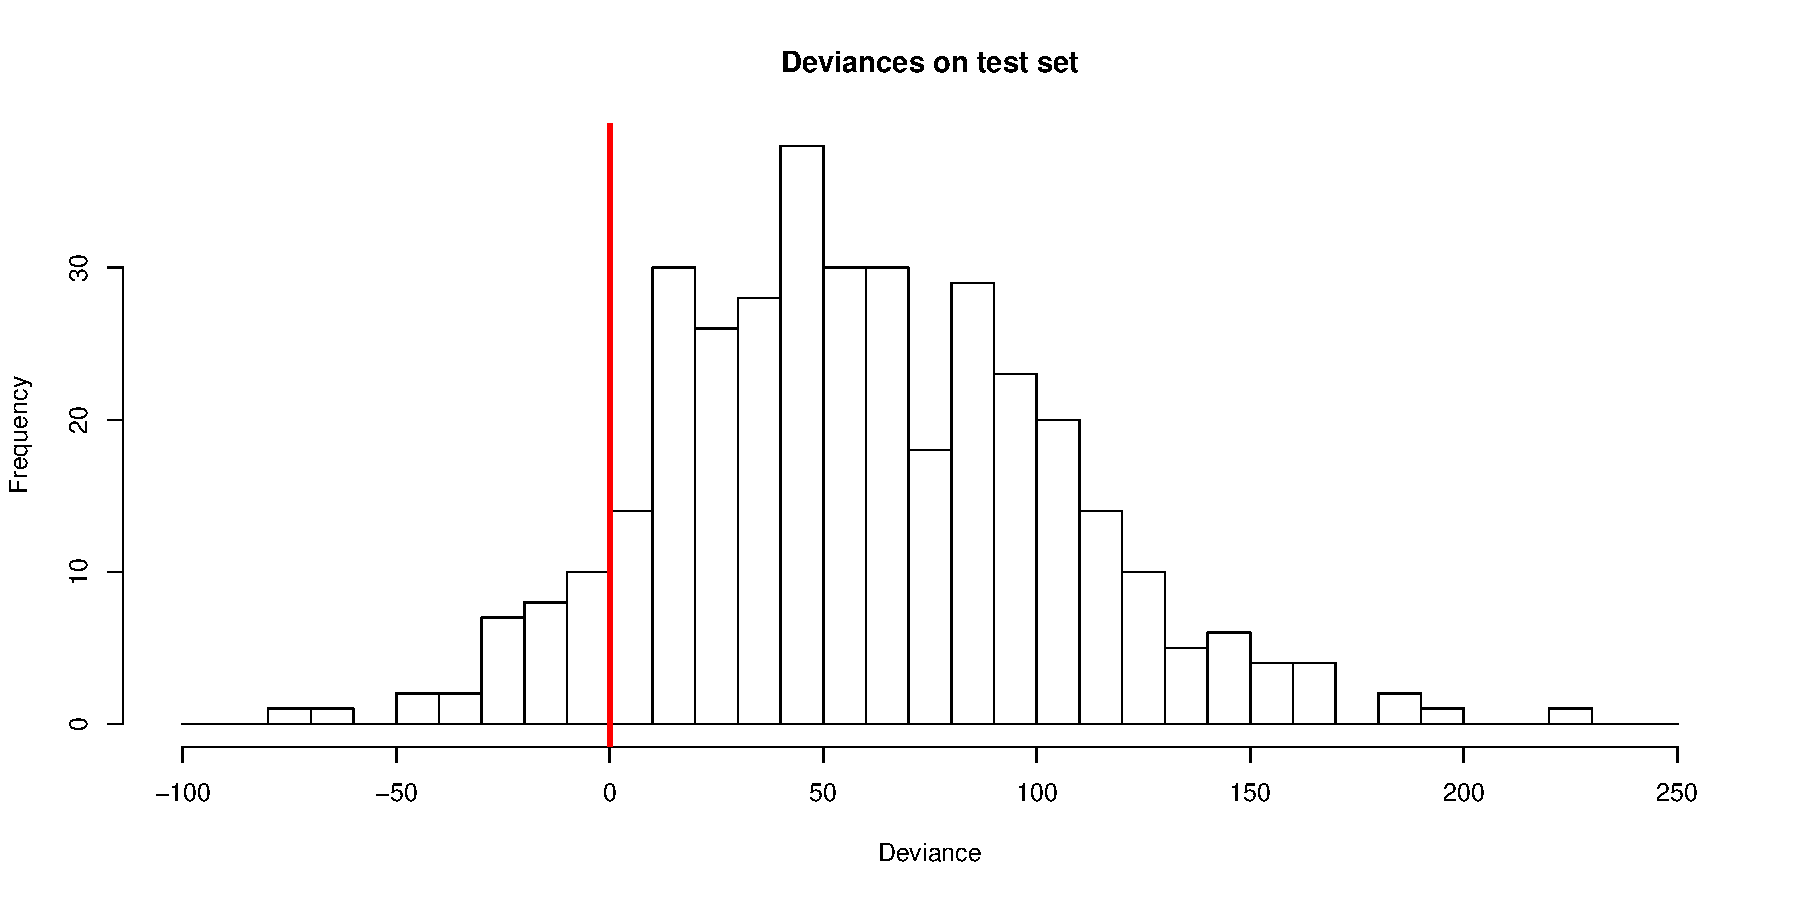
\includegraphics[scale=0.4]{figures/correlated_non-cyclic-no-intercept_cv_deviance.pdf}
\end{figure}